% =============================================================================
% EXERCICES
% =============================================================================

\section*{Exercices}
\addcontentsline{toc}{section}{Exercices}

\textbf{Données utiles :}
\begin{itemize}
    \item Accélération gravitationnelle : $g = 9{,}81$~m/s²
    \item Constante de gravitation : $G = 6{,}674 \times 10^{-11}$~N$\cdot$m²/kg²
    \item Masse de la Terre : $M_T = 5{,}972 \times 10^{24}$~kg
    \item Rayon de la Terre : $R_T = 6{,}378 \times 10^{6}$~m
    \item 1 nœud = 0,514 m/s
\end{itemize}

% -----------------------------------------------------------------------------
\subsection*{Dynamique -- Niveau 1 (Application directe)}
% -----------------------------------------------------------------------------

\begin{enumerate}

\item Une balle de fusil de 10~g qui se déplace à 400~m/s s'arrête après avoir pénétré de 3~cm dans un bloc de bois. Trouvez le module de la force agissant sur la balle, en la supposant constante.

\textit{Réponse : 26,7 kN}

\item \textbf{(Maritime)} Sur un quai, un treuil tire une caisse de 60~kg à l'aide d'un câble formant un angle de 20° au-dessus de l'horizontale. La tension dans le câble est de 440~N et la force de frottement entre la caisse et le quai est de 302~N.
\begin{enumerate}
    \item Quelle est la grandeur de la force normale?
    \item Quelle est l'accélération de la caisse?
\end{enumerate}

\textit{Réponses : a) 438 N \quad b) 1,85 m/s²}

\item \textbf{(Maritime)} Lorsqu'il n'est pas brisé, le F.A. Gauthier ($m = 5000$ tonnes métriques) peut passer de 0 à 10,0 nœuds en 120~s.
\begin{enumerate}
    \item En supposant que son accélération soit constante, déterminez la force de poussée de ses moteurs azimutaux. Négligez le frottement avec l'eau.
    \item Quelle est la force de frottement du navire avec l'eau si sa vitesse maximale est de 20 nœuds lorsque les moteurs fonctionnent à plein régime?
\end{enumerate}

\textit{Réponses : a) 214 kN \quad b) 214 kN}

\item \textbf{(Maritime)} Un conteneur de 10 tonnes est arrimé sur le pont d'un navire. Le navire décélère à raison de 0,6~m/s² lors d'une manœuvre d'urgence. Quelle est la force de frottement minimale requise pour que le conteneur ne glisse pas?

\textit{Réponse : 60 kN}

\end{enumerate}

% -----------------------------------------------------------------------------
\subsection*{Dynamique -- Niveau 2 (Plans inclinés et frottement)}
% -----------------------------------------------------------------------------

\begin{enumerate}[resume]

\item Le Père Noël tire son lourd traîneau (490~kg) afin de monter une pente bien glacée (frottement négligeable). L'angle de la pente est $\theta = 18°$ et l'angle de la corde par rapport à la pente est $\beta = 26°$.
\begin{enumerate}
    \item Quelle tension le Père Noël doit-il appliquer pour que le traîneau se déplace à vitesse constante?
    \item Quelle est l'accélération du traîneau si $T = 1$~kN?
\end{enumerate}

\textit{Réponses : a) 1,65 kN \quad b) 1,20 m/s² vers le bas de la pente}

\item \textbf{(Maritime)} Une palette de 200~kg glisse du repos sur une rampe de chargement inclinée à 35°. Après avoir parcouru 3~m sur la rampe, sa vitesse est de 1~m/s. Quelle était la force de frottement sur la rampe?

\textit{Réponse : 1090 N}

\item \textbf{(Maritime)} Un baril de 30~kg part du repos à une hauteur de 60~cm sur une rampe inclinée à 30° menant à la cale d'un navire. Un frottement de 51~N s'exerce pendant la descente, puis un frottement de 59~N sur le plancher horizontal de la cale. À quelle distance du bas de la rampe le baril s'immobilise-t-il?

\textit{Réponse : 1,96 m}

\item \textbf{(Maritime)} Une caisse de marchandise (400~kg) est sur une passerelle de navire inclinée à 35°. Quel est le coefficient de frottement statique minimal entre la caisse et la passerelle afin que la caisse ne glisse pas?

\textit{Réponse : 0,700}

\end{enumerate}

% -----------------------------------------------------------------------------
\subsection*{Dynamique -- Niveau 3 (Systèmes de poulies)}
% -----------------------------------------------------------------------------

\begin{enumerate}[resume]

\item \textbf{(Machine d'Atwood)} Deux masses ($m_1 = 4$~kg, $m_2 = 6$~kg) sont suspendues de part et d'autre d'une poulie de masse négligeable pouvant tourner sans frottement.
\begin{enumerate}
    \item Quelle est la tension dans la corde qui relie les deux masses?
    \item Quelle est l'accélération de chaque masse?
    \item Quelle est la vitesse du bloc $m_1$ après avoir monté de 1~m par rapport à sa position au repos?
    \item Quelle est la force que la poulie exerce sur le plafond?
\end{enumerate}

\textit{Réponses : a) 47,1 N \quad b) 1,96 m/s² \quad c) 1,98 m/s \quad d) 94,2 N}

\item \textbf{(Maritime)} Sur un quai, une caisse de 30~kg est reliée par une corde passant par une poulie à un contrepoids de 20~kg suspendu au-dessus de l'eau. La surface du quai est sans frottement.
\begin{enumerate}
    \item Quelle est l'accélération du système?
    \item Quelle est la tension dans la corde?
\end{enumerate}

\textit{Réponses : a) 3,92 m/s² \quad b) 118 N}

\item \textbf{(Maritime)} Lors du chargement d'un navire, une caisse de 50~kg est posée sur une rampe inclinée à 30° avec un coefficient de frottement cinétique $\mu_c = 0,2$. Elle est reliée par une corde passant par une poulie au sommet de la rampe à un contrepoids de 30~kg suspendu dans le vide. Si le système est relâché du repos :
\begin{enumerate}
    \item Dans quelle direction le système se met-il en mouvement?
    \item Quelle est l'accélération du système?
\end{enumerate}

\textit{Indice : Comparez le poids du contrepoids avec la composante du poids de la caisse parallèle à la rampe plus le frottement.}

\end{enumerate}

% -----------------------------------------------------------------------------
\subsection*{Mouvement circulaire}
% -----------------------------------------------------------------------------

\begin{enumerate}[resume]

\item Une automobile prend un virage horizontal de rayon 25~m. Le coefficient de frottement statique entre les pneus et la route est $\mu_s = 0,5$. Quelle est la vitesse maximale à laquelle l'automobile peut prendre ce virage sans déraper?

\textit{Réponse : 39,9 km/h}

\item Un satellite de 800~kg est en orbite circulaire autour de la Terre à une altitude de 400~km.
\begin{enumerate}
    \item Quelle est la force gravitationnelle agissant sur le satellite?
    \item Quelle est l'accélération gravitationnelle à cette altitude?
    \item À quelle vitesse tangentielle le satellite doit-il se déplacer pour conserver son orbite?
    \item En combien de temps ce satellite fait-il une révolution complète?
\end{enumerate}

\textit{Réponses : a) 7,38 kN \quad b) 9,23 m/s² \quad c) 27\,800 km/h \quad d) 92 min 21 s}

\item \textbf{(Maritime)} Un navire de croisière passe par le sommet d'une vague dont le profil a un rayon de courbure de 50~m. Quelle est la vitesse maximale du navire pour que les passagers restent en contact avec le pont?

\textit{Réponse : 79,8 km/h (43,1 nœuds)}

\item Quelle serait la durée d'un jour si une personne située à l'équateur avait un poids apparent nul? Le rayon moyen de la Terre est de 6378~km.

\textit{Réponse : 84 min 26 s}

\item Un enfant de 25~kg est assis sur un siège de manège qui tourne en cercle horizontal de rayon 4~m. Le siège est suspendu par des chaînes qui font un angle de 30° avec la verticale lorsque le manège tourne.
\begin{enumerate}
    \item Quelle est la vitesse du manège?
    \item Quelle est la tension dans les chaînes?
\end{enumerate}

\textit{Réponses : a) 4,75 m/s (17,1 km/h) \quad b) 283 N}

\item Une balle de 0,5~kg est attachée à une corde de 1,2~m et tourne en cercle horizontal (pendule conique). La corde fait un angle de 20° avec la verticale.
\begin{enumerate}
    \item Quelle est la vitesse de la balle?
    \item Quelle est la période de rotation?
\end{enumerate}

\textit{Réponses : a) 1,21 m/s \quad b) 2,13 s}

\end{enumerate}

% -----------------------------------------------------------------------------
\subsection*{Statique (Équilibre)}
% -----------------------------------------------------------------------------

Les figures suivantes accompagnent les problèmes de statique :

% ---- FIGURES 1 et 2 --------------------------------------------------------
\begin{center}
\begin{tikzpicture}[scale=0.85]
    % =====================================================================
    % FIGURE 1 — Trapéziste (angles 75° et 80° avec l'horizontale)
    % =====================================================================
    \begin{scope}[xshift=0cm]
        \node[above, font=\bfseries] at (0,4.2) {Figure 1};

        % --- Paramètres ---
        \pgfmathsetmacro{\aL}{75}  % angle gauche avec l'horizontale
        \pgfmathsetmacro{\aR}{80}  % angle droit avec l'horizontale
        \pgfmathsetmacro{\cLen}{3} % longueur visuelle des câbles

        % --- Coordonnées calculées ---
        \pgfmathsetmacro{\xL}{-\cLen*cos(\aL)}  % ≈ -0.78
        \pgfmathsetmacro{\yL}{\cLen*sin(\aL)}   % ≈ 2.90
        \pgfmathsetmacro{\xR}{\cLen*cos(\aR)}   % ≈ 0.52
        \pgfmathsetmacro{\yR}{\cLen*sin(\aR)}   % ≈ 2.95

        \coordinate (O) at (0,0);           % point de jonction
        \coordinate (L) at (\xL,\yL);       % ancrage gauche
        \coordinate (R) at (\xR,\yR);       % ancrage droit

        % --- Plafond ---
        \pgfmathsetmacro{\yPlaf}{max(\yL,\yR)}
        \fill[pattern=north east lines] (\xL-0.6,\yPlaf) rectangle (\xR+0.6,\yPlaf+0.3);
        \draw[thick] (\xL-0.6,\yPlaf) -- (\xR+0.6,\yPlaf);

        % --- Câbles ---
        \draw[thick] (L) -- (O) node[midway, left] {$T_1$};
        \draw[thick] (R) -- (O) node[midway, right] {$T_2$};

        % --- Références verticales (pointillées) et arcs d'angles ---
        % Gauche : 15° avec la verticale
        \draw[dashed, gray] (L) -- ++(0,-2);
        \pgfmathsetmacro{\arcStartL}{270}
        \pgfmathsetmacro{\arcEndL}{270 + (90-\aL)}  % 270 + 15 = 285
        \draw ([shift={(0,-0.7)}]L) arc (\arcStartL:\arcEndL:0.7);
        \node[font=\small] at ([shift={(0.35,-0.95)}]L) {$15°$};

        % Droite : 10° avec la verticale
        \draw[dashed, gray] (R) -- ++(0,-2);
        \pgfmathsetmacro{\arcStartR}{270}
        \pgfmathsetmacro{\arcEndR}{270 - (90-\aR)}  % 270 - 10 = 260
        \draw ([shift={(0,-0.7)}]R) arc (\arcStartR:\arcEndR:0.7);
        \node[font=\small] at ([shift={(-0.35,-0.95)}]R) {$10°$};

        % --- Trapéziste (personnage stylisé) ---
        \draw[thick, fill=gray!30] (O) circle (0.15);
        \draw[thick] (0,-0.15) -- (0,-0.9);        % tronc
        \draw[thick] (0,-0.4) -- (-0.3,-0.75);     % bras gauche
        \draw[thick] (0,-0.4) -- (0.3,-0.75);      % bras droit
        \draw[thick] (0,-0.9) -- (-0.2,-1.35);     % jambe gauche
        \draw[thick] (0,-0.9) -- (0.2,-1.35);      % jambe droite

        \node[below, font=\small] at (0,-1.55) {$m = 76$~kg};
    \end{scope}

    % =====================================================================
    % FIGURE 2 — Système de câbles au point C
    % =====================================================================
    \begin{scope}[xshift=9cm]
        \node[above, font=\bfseries] at (0,4.2) {Figure 2};

        % --- Paramètres ---
        \pgfmathsetmacro{\angAC}{25}  % angle de AC avec l'horizontale (depuis le mur)
        \pgfmathsetmacro{\angBC}{50}  % angle de BC avec la verticale (depuis le plafond)

        % --- Géométrie ---
        \coordinate (C) at (0,1.5);                   % point de jonction
        \pgfmathsetmacro{\xA}{-2.2}                   % mur à gauche
        \pgfmathsetmacro{\yA}{1.5 + 2.2*tan(\angAC)} % point A sur le mur
        \coordinate (A) at (\xA,\yA);
        \pgfmathsetmacro{\xB}{1.5*tan(\angBC)}        % point B au plafond
        \pgfmathsetmacro{\yB}{3.0}
        \coordinate (B) at (\xB,\yB);

        % --- Mur gauche ---
        \fill[pattern=north east lines] (-2.5,0) rectangle (-2.2,3.3);
        \draw[thick] (-2.2,0) -- (-2.2,3.3);

        % --- Plafond ---
        \fill[pattern=north east lines] (-2.2,3) rectangle (2.2,3.3);
        \draw[thick] (-2.2,3) -- (2.2,3);

        % --- Câbles ---
        \draw[thick] (A) -- (C) node[midway, above] {$T_{AC}$};
        \draw[thick] (B) -- (C) node[midway, right] {$T_{BC}$};
        \draw[thick] (C) -- (0,0);

        % --- Point C ---
        \filldraw[black] (C) circle (2.5pt) node[right=4pt] {C};

        % --- Référence horizontale pour angle AC et arc ---
        \draw[dashed, gray] (A) -- ++(1.5,0);
        \draw ([shift={(0.6,0)}]A) arc (0:\angAC:0.6);
        \node[font=\small] at ([shift={(1.0,0.3)}]A) {$25°$};

        % --- Référence verticale pour angle BC et arc ---
        \draw[dashed, gray] (B) -- ++(0,-1.5);
        \pgfmathsetmacro{\arcBCstart}{270}
        \pgfmathsetmacro{\arcBCend}{270-\angBC}  % 220
        \draw ([shift={(0,-0.6)}]B) arc (\arcBCstart:\arcBCend:0.6);
        \node[font=\small] at ([shift={(-0.5,-0.85)}]B) {$50°$};

        % --- Masse ---
        \draw[thick, fill=blue!20] (-0.4,-0.5) rectangle (0.4,0);
        \node at (0,-0.25) {\small $m$};
    \end{scope}
\end{tikzpicture}
\end{center}

% ---- FIGURES 3 et 4 --------------------------------------------------------
\begin{center}
\begin{tikzpicture}[scale=0.85]
    % =====================================================================
    % FIGURE 3 — Moteur suspendu (CORRIGÉE : 2 câbles de support)
    %   AB au plafond à 30° de l'horizontale, AD horizontal à la cloison
    %   Câble vertical de A vers le moteur
    % =====================================================================
    \begin{scope}[xshift=0cm]
        \node[above, font=\bfseries] at (0.5,4.2) {Figure 3};

        % --- Paramètres ---
        \pgfmathsetmacro{\angAB}{30}  % angle de AB avec l'horizontale
        \pgfmathsetmacro{\cabLen}{2.5} % longueur visuelle du câble AB

        % --- Coordonnées ---
        \coordinate (A) at (0,1.8);                        % point de jonction
        \pgfmathsetmacro{\xB}{-\cabLen*cos(\angAB)}       % ≈ -2.17
        \pgfmathsetmacro{\yB}{1.8 + \cabLen*sin(\angAB)}  % ≈ 3.05
        \coordinate (B) at (\xB,\yB);
        \coordinate (D) at (2.5,1.8);                      % cloison à droite

        % --- Plafond ---
        \fill[pattern=north east lines] (\xB-0.3,3.3) rectangle (2.5,3.6);
        \draw[thick] (\xB-0.3,3.3) -- (2.5,3.3);

        % --- Cloison droite ---
        \fill[pattern=north east lines] (2.5,0) rectangle (2.8,3.6);
        \draw[thick] (2.5,0) -- (2.5,3.6);

        % --- Câble AB (plafond, 30° avec l'horizontale) ---
        \draw[thick] (B) -- (A) node[midway, above left] {$T_{AB}$};

        % --- Câble AD (horizontal, cloison) ---
        \draw[thick] (A) -- (D) node[midway, above] {$T_{AD}$};

        % --- Câble vertical A → moteur ---
        \draw[thick] (A) -- (0,0.8);

        % --- Point A ---
        \filldraw[black] (A) circle (2.5pt) node[left=4pt] {A};

        % --- Labels des points d'ancrage ---
        \node[above left, font=\small] at (B) {B};
        \node[right, font=\small] at (2.5,1.8) {D};

        % --- Référence horizontale et arc d'angle pour AB ---
        \draw[dashed, gray] (A) -- ++(-2,0);
        \draw ([shift={(-0.7,0)}]A) arc (180:{180-\angAB}:0.7);
        \node[font=\small] at ([shift={(-1.1,0.35)}]A) {$30°$};

        % --- Moteur ---
        \draw[thick, fill=gray!40] (-0.5,0) rectangle (0.5,0.8);
        \node at (0,0.4) {M};
        \node[below, font=\small] at (0,-0.2) {250~kg};
    \end{scope}

    % =====================================================================
    % FIGURE 4 — Caisse sur quai + poulie + conteneur suspendu
    % =====================================================================
    \begin{scope}[xshift=9cm]
        \node[above, font=\bfseries] at (1.5,4.2) {Figure 4};

        % --- Paramètres ---
        \pgfmathsetmacro{\angCable}{35}  % angle du câble avec l'horizontale
        \pgfmathsetmacro{\rPoulie}{0.3}  % rayon de la poulie

        % --- Coordonnées principales ---
        \coordinate (caisse) at (-0.5,0.4);       % centre de la caisse
        \coordinate (coinCaisse) at (0.1,0.6);    % point d'attache sur la caisse
        \coordinate (Ppoulie) at (3.0,2.8);       % centre de la poulie

        % --- Surface du quai ---
        \fill[pattern=north east lines] (-2.0,-0.2) rectangle (3.5,0);
        \draw[thick] (-2.0,0) -- (3.5,0);

        % --- Bord du quai (vertical) ---
        \draw[thick] (3.5,0) -- (3.5,-1.5);
        \fill[pattern=north east lines] (3.5,-1.5) rectangle (3.8,0);

        % --- Eau ---
        \draw[blue!40, thick, decorate, decoration={snake, amplitude=1.5pt, segment length=8pt}]
            (2.0,-1.5) -- (3.5,-1.5);

        % --- Caisse 30 kg sur le quai ---
        \draw[thick, fill=blue!20] (-1.1,0) rectangle (0.1,0.8);
        \node[font=\small] at (-0.5,0.4) {30 kg};

        % --- Support de la poulie ---
        \draw[thick, gray] (3.5,2.3) -- (3.0,2.8);  % bras
        \fill[pattern=north east lines] (3.3,2.0) rectangle (3.7,2.3);
        \draw[thick] (3.3,2.3) -- (3.7,2.3);

        % --- Poulie ---
        \draw[thick, fill=white] (Ppoulie) circle (\rPoulie);
        \filldraw[black] (Ppoulie) circle (1.5pt);

        % --- Câble : caisse → poulie (angle 35° avec l'horizontale) ---
        \pgfmathsetmacro{\xTang}{3.0 - \rPoulie*sin(\angCable)}
        \pgfmathsetmacro{\yTang}{2.8 - \rPoulie*cos(\angCable)}
        \draw[thick] (coinCaisse) -- (\xTang,\yTang);

        % --- Câble : poulie → conteneur (vertical) ---
        \draw[thick] ({3.0 + \rPoulie},2.8) -- (3.3,0.8);

        % --- Conteneur 40 kg suspendu ---
        \draw[thick, fill=red!20] (2.9,0.1) rectangle (3.7,0.8);
        \node[font=\small] at (3.3,0.45) {40 kg};

        % --- Câble de retenue horizontal → bollard ---
        \draw[thick] (-1.1,0.4) -- (-1.8,0.4);
        % Bollard
        \draw[thick, fill=gray!60] (-1.8,0) -- (-1.8,0.55) -- (-2.0,0.55)
            -- (-2.0,0.45) -- (-1.9,0.45) -- (-1.9,0) -- cycle;
        \node[font=\small, above] at (-1.9,0.6) {bollard};
        \node[font=\small, below] at (-1.5,0.25) {$T_{ret}$};

        % --- Arc d'angle 35° avec référence horizontale ---
        \draw[dashed, gray] (coinCaisse) -- ++(2,0);
        \draw ([shift={(0.7,0)}]coinCaisse) arc (0:\angCable:0.7);
        \node[font=\small] at ([shift={(1.0,0.35)}]coinCaisse) {$35°$};
    \end{scope}
\end{tikzpicture}
\end{center}

% ---- FIGURE 5 --------------------------------------------------------------
\begin{center}
\begin{tikzpicture}[scale=0.85]
    % =====================================================================
    % FIGURE 5 — Deux matelots soulèvent une caisse via un crochet
    %   Câble gauche : 10° avec la verticale
    %   Câble droite : 55° avec la verticale
    % =====================================================================
    \node[above, font=\bfseries] at (0,4.5) {Figure 5};

    % --- Paramètres ---
    \pgfmathsetmacro{\angL}{10}   % angle gauche avec la verticale
    \pgfmathsetmacro{\angR}{55}   % angle droit avec la verticale
    \pgfmathsetmacro{\cabLen}{2.8} % longueur visuelle des câbles

    % --- Point de jonction (sous le crochet) ---
    \coordinate (J) at (0,1.2);

    % --- Plafond de la cale ---
    \fill[pattern=north east lines] (-3.5,4.0) rectangle (3.5,4.3);
    \draw[thick] (-3.5,4.0) -- (3.5,4.0);

    % --- Crochet au plafond ---
    \draw[thick] (0,4.0) -- (0,3.5);
    \draw[thick, fill=gray!50] (0,3.5) arc (0:-180:0.15) -- cycle;
    \filldraw[black] (0,3.5) circle (1.5pt);

    % --- Câble vertical du crochet vers le point de jonction ---
    \draw[thick] (0,3.35) -- (J);

    % --- Coordonnées des matelots ---
    \pgfmathsetmacro{\xL}{-\cabLen*sin(\angL)}   % ≈ -0.49
    \pgfmathsetmacro{\yL}{1.2 + \cabLen*cos(\angL)}  % ≈ 3.96
    \pgfmathsetmacro{\xR}{\cabLen*sin(\angR)}    % ≈ 2.29
    \pgfmathsetmacro{\yR}{1.2 + \cabLen*cos(\angR)}  % ≈ 2.81

    \coordinate (L) at (\xL,\yL);  % matelot gauche (en haut)
    \coordinate (R) at (\xR,\yR);  % matelot droite

    % --- Câbles vers les matelots ---
    \draw[thick] (J) -- (L) node[midway, left] {$T_1$};
    \draw[thick] (J) -- (R) node[midway, right] {$T_2$};

    % --- Flèches de tension (indiquant la direction de traction) ---
    \draw[->, very thick, blue] (J) -- ++({-1.2*sin(\angL)},{1.2*cos(\angL)});
    \draw[->, very thick, red] (J) -- ++({1.2*sin(\angR)},{1.2*cos(\angR)});

    % --- Référence verticale et arcs d'angles ---
    % Verticale de référence
    \draw[dashed, gray] (J) -- ++(0,3.2);

    % Arc gauche (10° avec la verticale)
    \draw (0,{1.2+0.8}) arc (90:{90+\angL}:0.8);
    \node[font=\small] at (-0.35,2.25) {$10°$};

    % Arc droit (55° avec la verticale)
    \draw (0,{1.2+0.8}) arc (90:{90-\angR}:0.8);
    \node[font=\small] at (0.65,1.85) {$55°$};

    % --- Point de jonction ---
    \filldraw[black] (J) circle (2.5pt);

    % --- Câble vertical vers la caisse ---
    \draw[thick] (J) -- (0,0.5);

    % --- Caisse ---
    \draw[thick, fill=blue!20] (-0.5,-0.1) rectangle (0.5,0.5);
    \node[font=\small] at (0,0.2) {$m = {?}$};

    % --- Label de la tension connue ---
    \node[font=\small, blue, left] at ({-0.49-0.3},{3.2}) {200 N};
\end{tikzpicture}
\end{center}

\begin{enumerate}[resume]

\item Une trapéziste suspendue à un câble a une masse de 76~kg. Le câble de gauche fait un angle de 75° avec l'horizontale (15° avec la verticale) et celui de droite fait un angle de 80° avec l'horizontale (10° avec la verticale) (Figure 1). Déterminez les tensions $T_1$ et $T_2$.

\textit{Réponses : $T_1 = 306$ N ; $T_2 = 457$ N}

\item \textbf{(Maritime)} Un moteur diesel de 250~kg est suspendu au point de jonction A par un câble vertical dans la salle des machines d'un navire (Figure 3). Au point A, deux câbles maintiennent le système en équilibre : le câble AB est fixé au plafond et fait un angle de 30° avec l'horizontale, tandis que le câble AD est horizontal et fixé à la cloison.
\begin{enumerate}
    \item Déterminez la tension dans les câbles AB et AD.
    \item La composante verticale de la tension dans le câble AB suffit à supporter le poids du moteur. Pourquoi le câble AD est-il nécessaire?
\end{enumerate}

\textit{Réponses : a) $T_{AB} = 4{,}90$~kN ; $T_{AD} = 4{,}24$~kN}

\item \textbf{(Maritime)} Sur un quai, une caisse de 30~kg est posée sur une surface sans frottement (Figure 4). Un câble attaché à la caisse passe par une poulie fixée en hauteur au bord du quai, puis descend verticalement pour supporter un conteneur de 40~kg au-dessus de l'eau. Le segment de câble entre la caisse et la poulie fait un angle de 35° avec l'horizontale. Un câble de retenue horizontal, attaché à un bollard, maintient la caisse en équilibre.
\begin{enumerate}
    \item Déterminez la tension dans le câble de retenue.
    \item Quelle est la force normale exercée par le quai sur la caisse?
\end{enumerate}

\textit{Réponses : a) $T_{ret} = 321$ N \quad b) $N = 69{,}2$ N}

\item \textbf{(Maritime)} Deux matelots soulèvent une caisse à l'aide de câbles passant par un crochet fixé au plafond de la cale (Figure 5). Au point de jonction sous le crochet, le câble de gauche fait un angle de 10° avec la verticale et le câble de droite fait un angle de 55° avec la verticale. Le matelot de gauche exerce une tension de 200~N.
\begin{enumerate}
    \item Déterminez la tension exercée par le matelot de droite.
    \item Quelle est la masse de la caisse?
\end{enumerate}

\textit{Réponses : a) $T_2 = 42{,}4$~N \quad b) $m = 22{,}6$~kg}

\end{enumerate}

% -----------------------------------------------------------------------------
\subsection*{Problèmes de synthèse}
% -----------------------------------------------------------------------------

\begin{center}
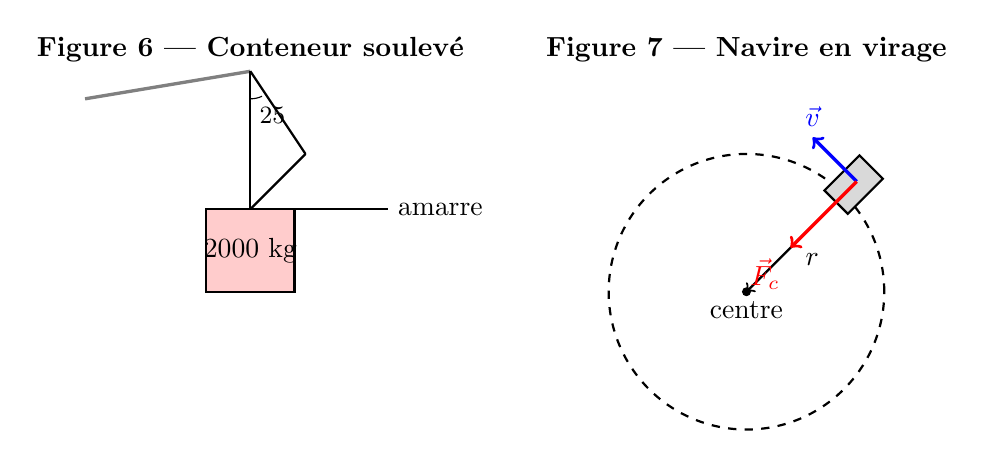
\begin{tikzpicture}[scale=0.7]
    % FIGURE 6 - Conteneur avec grue
    \begin{scope}[xshift=0cm]
        \node[above] at (0,4) {\textbf{Figure 6 — Conteneur soulevé}};
        
        % Grue (bras)
        \draw[very thick, gray] (-3,3.5) -- (0,4);
        
        % Câble de grue (incliné)
        \draw[thick] (0,4) -- (0,1.5);
        \draw[thick] (0,4) -- (1,2.5);
        \draw[thick] (1,2.5) -- (0,1.5);
        
        % Angle
        \draw (0,3.5) arc (270:295:0.5);
        \node at (0.4,3.2) {\small $25°$};
        
        % Amarre horizontale
        \draw[thick] (0,1.5) -- (2.5,1.5);
        \node[right] at (2.5,1.5) {amarre};
        
        % Conteneur
        \draw[thick, fill=red!20] (-0.8,0) rectangle (0.8,1.5);
        \node at (0,0.75) {2000 kg};
    \end{scope}
    
    % FIGURE 7 - Navire en virage (vue de dessus)
    \begin{scope}[xshift=9cm]
        \node[above] at (0,4) {\textbf{Figure 7 — Navire en virage}};
        
        % Arc de cercle (virage)
        \draw[thick, dashed] (0,0) circle (2.5);
        
        % Centre
        \filldraw[black] (0,0) circle (2pt) node[below] {centre};
        
        % Rayon
        \draw[<->, thick] (0,0) -- (1.77,1.77) node[midway, below right] {$r$};
        
        % Navire
        \draw[thick, fill=gray!30, rotate=45] (2.3,-0.3) rectangle (3.2,0.3);
        
        % Vitesse
        \draw[->, very thick, blue] (2,2) -- (1.2,2.8) node[above] {$\vec{v}$};
        
        % Force centripète
        \draw[->, very thick, red] (2,2) -- (0.8,0.8) node[below left] {$\vec{F}_c$};
    \end{scope}
\end{tikzpicture}
\end{center}

\begin{enumerate}[resume]

\item \textbf{(Contexte maritime — Figure 6)} Un conteneur de 2000~kg est soulevé par une grue à bord d'un navire. Le câble de la grue fait un angle de 25° avec la verticale. Une amarre horizontale est attachée au conteneur pour l'empêcher de balancer.
\begin{enumerate}
    \item Tracez le DCL du conteneur.
    \item Calculez la tension dans le câble de la grue.
    \item Calculez la tension dans l'amarre horizontale.
\end{enumerate}

\textit{Réponses : b) $T = 21{,}6$~kN \quad c) $T_h = 9{,}14$~kN}

\item \textbf{(Contexte maritime — Figure 7)} Un navire de 15\,000 tonnes effectue un virage de rayon 800~m à une vitesse de 12 nœuds.
\begin{enumerate}
    \item Quelle force centripète est nécessaire pour ce virage?
    \item Cette force est fournie par la résistance latérale de l'eau sur la coque. Si cette résistance maximale est de 500~kN, quelle est la vitesse maximale à laquelle le navire peut effectuer ce virage?
\end{enumerate}

\textit{Réponses : a) $F_c = 714$~kN \quad b) $v_{max} = 14{,}7$~nœuds}

\item \textbf{(Problème combiné)} Une caisse de 50~kg est posée sur le pont d'un navire. Le coefficient de frottement statique entre la caisse et le pont est $\mu_s = 0,35$.
\begin{enumerate}
    \item Si le navire accélère en ligne droite, quelle est l'accélération maximale avant que la caisse ne glisse?
    \item Si le navire effectue un virage à vitesse constante de 8 nœuds, quel est le rayon minimal du virage pour que la caisse ne glisse pas?
\end{enumerate}

\textit{Réponses : a) $a_{max} = 3{,}43$~m/s² \quad b) $r_{min} = 4{,}93$~m}

\end{enumerate}

% -----------------------------------------------------------------------------
\subsection*{Mouvement circulaire — Applications maritimes}
% -----------------------------------------------------------------------------

\begin{center}
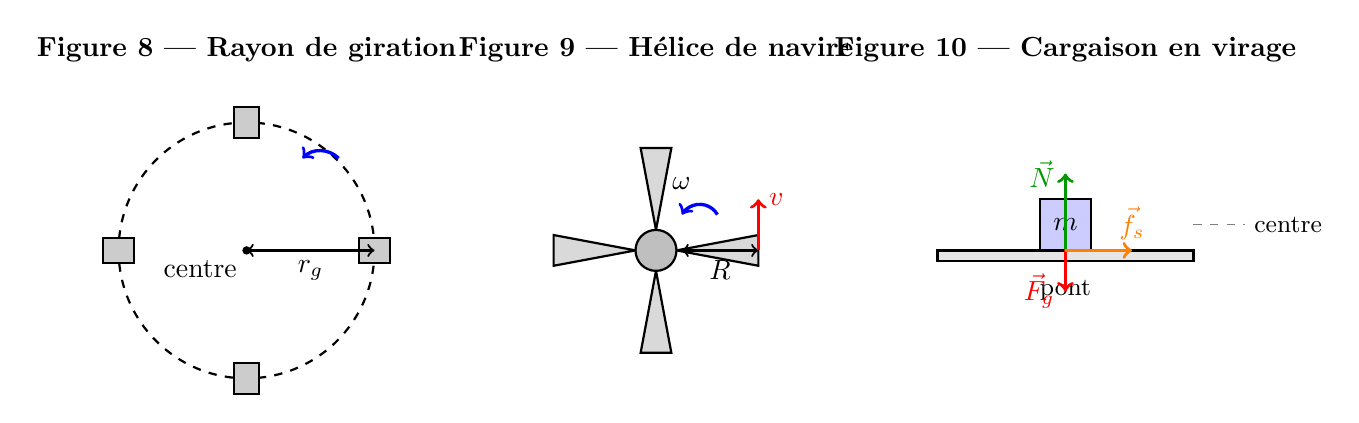
\begin{tikzpicture}[scale=0.65]
    % FIGURE 8 - Rayon de giration
    \begin{scope}[xshift=0cm]
        \node[above] at (0,3.5) {\textbf{Figure 8 — Rayon de giration}};
        
        % Cercle de virage
        \draw[thick, dashed] (0,0) circle (2.5);
        
        % Point central
        \filldraw[black] (0,0) circle (2pt);
        \node[below left] at (0,0) {centre};
        
        % Navire à différentes positions
        \draw[thick, fill=gray!40, rotate=90] (2.2,-0.25) rectangle (2.8,0.25);
        \draw[thick, fill=gray!40, rotate=180] (2.2,-0.25) rectangle (2.8,0.25);
        \draw[thick, fill=gray!40, rotate=270] (2.2,-0.25) rectangle (2.8,0.25);
        \draw[thick, fill=gray!40, rotate=0] (2.2,-0.25) rectangle (2.8,0.25);
        
        % Rayon de giration
        \draw[<->, thick] (0,0) -- (2.5,0) node[midway, below] {$r_g$};
        
        % Flèche rotation
        \draw[->, very thick, blue] (1.8,1.8) arc (45:135:0.5);
    \end{scope}
    
    % FIGURE 9 - Hélice (corrigée)
    \begin{scope}[xshift=8cm]
        \node[above] at (0,3.5) {\textbf{Figure 9 — Hélice de navire}};
        
        % Hub central
        \draw[thick, fill=gray!50] (0,0) circle (0.4);
        
        % Pales (4 pales)
        \draw[thick, fill=gray!30, rotate=0] (0.4,0) -- (2,0.3) -- (2,-0.3) -- (0.4,0);
        \draw[thick, fill=gray!30, rotate=90] (0.4,0) -- (2,0.3) -- (2,-0.3) -- (0.4,0);
        \draw[thick, fill=gray!30, rotate=180] (0.4,0) -- (2,0.3) -- (2,-0.3) -- (0.4,0);
        \draw[thick, fill=gray!30, rotate=270] (0.4,0) -- (2,0.3) -- (2,-0.3) -- (0.4,0);
        
        % Rayon (du centre vers l'extrémité d'une pale - vers la droite)
        \draw[<->, thick] (0.5,0) -- (2,0) node[midway, below] {$R$};
        
        % Vitesse tangentielle à l'extrémité (perpendiculaire au rayon = vers le haut)
        \draw[->, very thick, red] (2,0) -- (2,1) node[right] {$v$};
        
        % Rotation (sens antihoraire)
        \draw[->, very thick, blue] (1.2,0.7) arc (30:150:0.4);
        \node at (0.5,1.3) {$\omega$};
    \end{scope}
    
    % FIGURE 10 - Cargaison dans virage (corrigée - forces au bon endroit)
    \begin{scope}[xshift=16cm]
        \node[above] at (0,3.5) {\textbf{Figure 10 — Cargaison en virage}};
        
        % Pont du navire
        \draw[thick, fill=gray!20] (-2.5,-0.2) rectangle (2.5,0);
        \node[below] at (0,-0.4) {\small pont};
        
        % Caisse
        \draw[thick, fill=blue!20] (-0.5,0) rectangle (0.5,1);
        \node at (0,0.5) {$m$};
        
        % Centre du virage (à droite)
        \draw[dashed, gray] (2.5,0.5) -- (3.5,0.5);
        \node[right] at (3.5,0.5) {\small centre};
        
        % DCL de la caisse (forces appliquées correctement)
        % Poids: au centre de masse, vers le bas
        \draw[->, very thick, red] (0,0.5) -- (0,-0.8) node[left] {$\vec{F}_g$};
        % Normale: à la base (contact avec le pont), vers le haut
        \draw[->, very thick, green!60!black] (0,0) -- (0,1.5) node[left] {$\vec{N}$};
        % Frottement: à la base, vers le centre du virage (vers la droite)
        \draw[->, very thick, orange] (0,0) -- (1.3,0) node[above] {$\vec{f}_s$};
    \end{scope}
\end{tikzpicture}
\end{center}

\begin{enumerate}[resume]

\item \textbf{(Rayon de giration — Figure 8)} Un pétrolier de 80\,000 tonnes métriques effectue un virage avec un rayon de giration de 600~m. Sa vitesse est de 15 nœuds.
\begin{enumerate}
    \item Quelle est la force centripète nécessaire pour maintenir ce virage?
    \item En combien de temps le navire effectue-t-il un virage de 180°?
    \item Si le capitaine réduit la vitesse à 10 nœuds, quelle sera la nouvelle force centripète?
\end{enumerate}

\textit{Réponses : a) $F_c = 7{,}93$~MN \quad b) $t = 4$~min~5~s \quad c) $F_c = 3{,}53$~MN}

\item \textbf{(Hélice — Figure 9)} L'hélice d'un navire a un diamètre de 6~m et tourne à 120~RPM.
\begin{enumerate}
    \item Quelle est la vitesse angulaire de l'hélice en rad/s?
    \item Quelle est la vitesse linéaire de l'extrémité des pales?
    \item Quelle est l'accélération centripète subie par un point à l'extrémité d'une pale?
\end{enumerate}

\textit{Réponses : a) $\omega = 12{,}6$~rad/s \quad b) $v = 37{,}7$~m/s (136 km/h) \quad c) $a_c = 474$~m/s²}

\item \textbf{(Cargaison en virage — Figure 10)} Un conteneur de 12 tonnes est arrimé sur le pont d'un navire. Le coefficient de frottement statique entre le conteneur et le pont est $\mu_s = 0{,}45$.
\begin{enumerate}
    \item Si le navire effectue un virage de rayon 500~m, quelle est la vitesse maximale pour que le conteneur ne glisse pas?
    \item À 8 nœuds, quel est le rayon de virage minimal sécuritaire?
\end{enumerate}

\textit{Réponses : a) $v_{max} = 28{,}9$~nœuds \quad b) $r_{min} = 3{,}84$~m}

\item \textbf{(Manœuvre d'urgence)} Un traversier de 5000 tonnes navigue à 18 nœuds et doit effectuer un virage d'urgence. La force latérale maximale que l'eau peut exercer sur la coque est de 800~kN.
\begin{enumerate}
    \item Quel est le rayon de virage minimal possible?
    \item Si le capitaine veut un rayon de 400~m, à quelle vitesse maximale peut-il effectuer le virage?
    \item Combien de temps faudra-t-il pour effectuer un demi-tour (180°) au rayon minimal?
\end{enumerate}

\textit{Réponses : a) $r_{min} = 535$~m \quad b) $v_{max} = 15{,}6$~nœuds \quad c) $t = 3$~min~2~s}

\item \textbf{(Câble de remorquage)} Un remorqueur tire un barge de 2000 tonnes en effectuant un virage de rayon 300~m à une vitesse de 6 nœuds. La tension dans le câble de remorquage doit fournir à la fois :
\begin{itemize}
    \item La force de propulsion : 50~kN (pour vaincre la résistance de l'eau)
    \item La force centripète nécessaire au virage
\end{itemize}
\begin{enumerate}
    \item Quelle force centripète est nécessaire pour maintenir la barge dans le virage?
    \item Quelle doit être la tension totale dans le câble si celui-ci est orienté vers le centre du virage? (Considérez que les deux forces s'ajoutent vectoriellement.)
\end{enumerate}

\textit{Réponses : a) $F_c = 63{,}5$~kN \quad b) $T = 80{,}9$~kN}

\item \textbf{(Stabilité en mer agitée)} Une bouée météorologique de 500~kg est attachée à son ancrage. Elle subit un mouvement circulaire vertical dû aux vagues. L'amplitude du mouvement est de 3~m et la période des vagues est de 8~s.
\begin{enumerate}
    \item Quelle est la vitesse maximale de la bouée?
    \item Quelle est l'accélération centripète maximale?
    \item À quel moment du cycle la tension dans le câble d'ancrage est-elle maximale? Quelle est cette tension?
\end{enumerate}

\textit{Réponses : a) $v_{max} = 2{,}36$~m/s \quad b) $a_c = 1{,}85$~m/s² \quad c) Au point le plus bas; $T_{max} = 5{,}83$~kN}

\end{enumerate}

% -----------------------------------------------------------------------------
% PRATIQUE AUTONOME DE SYNTHÈSE
% -----------------------------------------------------------------------------

\begin{pratiqueautonome}[title=Pratique autonome de synthèse — Manœuvre de navire]
Le traversier \textit{Saaremaa I} ($m = 8500$ tonnes) quitte le port de Rimouski à destination de Forestville. Pendant la traversée :

\begin{enumerate}
    \item Le navire accélère de 0 à 12 nœuds en 90 secondes. Quelle force de poussée les moteurs doivent-ils fournir? (Négligez la résistance de l'eau.)
    
    \item À vitesse constante de 12 nœuds, le navire effectue un virage de rayon 400~m. Quelle force centripète l'eau doit-elle exercer sur la coque?
    
    \item Sur le pont, un véhicule de 1800~kg n'est pas arrimé. Quel est le coefficient de frottement statique minimal requis pour qu'il ne glisse pas pendant le virage?
    
    \item Si une bourrasque de vent exerce une force latérale supplémentaire de 50~kN sur le navire pendant le virage, le véhicule glissera-t-il? ($\mu_s = 0{,}45$ entre les pneus et le pont)
\end{enumerate}

\vspace{4cm}

\tcblower
\textit{Réponses :}
\begin{enumerate}
    \item $F = 583$~kN
    \item $F_c = 810$~kN  
    \item $\mu_{s,min} = 0{,}097$
    \item Force sur le véhicule : $F_{vent/véhicule} = 50 \times \frac{1800}{8{,}5 \times 10^6} = 10{,}6$~N (négligeable). Force centripète requise : 172~N. Force de frottement max disponible : $0{,}45 \times 1800 \times 9{,}81 = 7{,}95$~kN. Non, le véhicule ne glissera pas.
\end{enumerate}
\end{pratiqueautonome}